\chapter*{Introduction} % Grammarly OK

In a world with an increasing number of electronic systems in hazardous environments, the correct operation of embedded systems is ever more important for ensuring fewer catastrophes. In the year 2000, Air France Concorde flight crashed soon after its take-off killing 113 people, in 2005 Texas City refinery exploded killing 15 people and injuring 180. Similar disasters were the motivation for the standardization of functional safety principles. 

\begin{figure}[H]
    \centering
    \begin{minipage}{.5\textwidth}
          \centering
          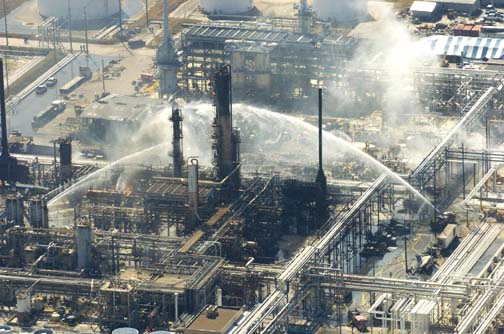
\includegraphics[width=.7\linewidth]{images/texas_refinery.jpg}
          \captionof{figure}{Texas refinery disaster \citep{texas_refinery_disaster}}
          \label{fig:texas_refinery}
    \end{minipage}%
    \begin{minipage}{.5\textwidth}
          \centering
          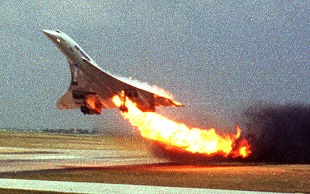
\includegraphics[width=.74\linewidth]{images/concorde_disaster.jpg}
          \captionof{figure}{ Air France Concorde disaster \citep{concorde_disaster}}
          \label{fig:concorde_disaster}
    \end{minipage}
\end{figure}

Functional safety is the part of the overall safety that depends on a system or equipment operating correctly in response to its inputs \cite{func_safety_brief}. In other words, the goal of functional safety is ensuring that even when the system fails its response is predictable and safe. Today, the concept of functional safety is part of everyday life and applies to almost every industry. For example, functional safety ensures that airbags in a car instantly deploy during impact to protect the passengers. Another good example is an automated flight control system in the airplanes. Autopilot controls the pitch and roll of the aircraft changing the heading and altitude, all of which is developed with respect to functional safety parameters, activating alarms and other measures when they are breached \cite{func_safety_brief}.

This paper explores how are principles of functional safety applied to engineering projects. How and why redundancy is implemented in hardware and software is investigated. As a part of that, redundant microcontrollers are explored and compared to non-redundant ones. Additionally, redundancy additions to the FreeRTOS operating system are implemented. Modifications add task replication and an option to measure the execution time of tasks. Finally, a secure bootloader is added, bootloader has a command shell interface and has the option of updating the current application.

\noindent The thesis is organized in the following way:

\begin{itemize}

    \item \autoref{functional_safety} gives brief introduction of functional safety and its certification process. Moreover, the chapter gives an overview of how is the hardware of embedded systems designed to support redundancy,
    \item \autoref{cortex_r_additions} investigates ARM Cortex-R microcontroller's architecture and what does is add over Cortex M,
    \item \autoref{freertos_kernel} gives an overview of FreeRTOS and implementation of tasks, scheduler and timers,
    \item \autoref{freertos_modification} gives an overview of added redundancy API to the FreeRTOS kernel,
    \item \autoref{custom_bootloader} explains the developed secure bootloader's architecture and
    \item \autoref{demonstration} demonstrates the functionality of the developed software.
    
\end{itemize}
   